\documentclass[11pt,oneside]{article}
\usepackage[T1]{fontenc}
\usepackage[utf8]{inputenc}
% \usepackage{lmodern}
%\usepackage[adobe-utopia,uppercase=upright,greeklowercase=upright]{mathdesign}
\usepackage[adobe-utopia]{mathdesign}
%\usepackage{minionpro}
% \usepackage{pifont}
% \usepackage{amssymb}
\usepackage{amsmath}
\usepackage[francais]{babel}
% \usepackage[francais]{varioref}
\usepackage[dvips]{graphicx}

\usepackage{framed}
\usepackage[normalem]{ulem}
\usepackage{fancyhdr}
\usepackage{titlesec}
\usepackage{vmargin}
\usepackage{longtable}

\usepackage{ifthen}


%\usepackage{epsfig}
\usepackage{subfig}

\usepackage{multirow}
\usepackage{multicol} % Portions de texte en colonnes
\usepackage{flafter}%floatants après la référence



\usepackage{color}
\usepackage{colortbl}


\definecolor{gris25}{gray}{0.75}
\definecolor{bleu}{RGB}{18,33,98}
\definecolor{bleuf}{RGB}{42,94,171}
\definecolor{bleuc}{RGB}{231,239,247}
\definecolor{rougef}{RGB}{185,18,27}
\definecolor{rougec}{RGB}{255,230,231}
\definecolor{vertf}{RGB}{103,126,82}
\definecolor{vertc}{RGB}{220,255,191}
\definecolor{violetf}{RGB}{112,48,160}
\definecolor{violetc}{RGB}{230,224,236}

\newenvironment{sci}[1][\hsize]%
{%
    \def\FrameCommand%
    {%
%\rotatebox{90}{\textit{\textsf{Scilab}}\includegraphics[height=.8cm]{png/logo_scilab}} 
\rotatebox{90}{\includegraphics[height=.6cm]{png/logo_scilab}} 
        {\color{violetf}\vrule width 3pt}%
        \hspace{0pt}%must no space.
        \fboxsep=\FrameSep\colorbox{violetc}%
    }%
    \MakeFramed{\hsize #1 \advance\hsize-\width\FrameRestore}%
}%
{\endMakeFramed}%

\newenvironment{pseudo}[1][\hsize]%
{%
    \def\FrameCommand%
    {%
\rotatebox{90}{\textit{\textsf{Pseudo Code}}} 
        {\color{violetf}\vrule width 3pt}%
        \hspace{0pt}%must no space.
        \fboxsep=\FrameSep\colorbox{violetc}%
    }%
    \MakeFramed{\hsize #1 \advance\hsize-\width\FrameRestore}%
}%
{\endMakeFramed}%

\newenvironment{py}[1][\hsize]%
{%
    \def\FrameCommand%
    {%
%\rotatebox{90}{\textit{\textsf{Python}}} 
\rotatebox{90}{\includegraphics[height=.6cm]{png/logo_python}} 
        {\color{violetf}\vrule width 3pt}%
        \hspace{0pt}%must no space.
        \fboxsep=\FrameSep\colorbox{violetc}%
    }%
    \MakeFramed{\hsize #1 \advance\hsize-\width\FrameRestore}%
}%
{\endMakeFramed}%


\newenvironment{corrige}[1][\hsize]%
{%
    \def\FrameCommand
    {%
\rotatebox{90}{\textit{\textsf{Correction}}} 
        {\color{violetf}\vrule width 3pt}%
        \hspace{0pt}%must no space.
        \fboxsep=\FrameSep\colorbox{violetc}%
    }%
    \MakeFramed{\hsize#1\advance\hsize-\width\FrameRestore}%
}%
{\endMakeFramed}%



\newenvironment{rem}[1][\hsize]%
{%
    \def\FrameCommand
    {%
\rotatebox{90}{\textit{\textsf{Remarque}}} 
        {\color{bleuf}\vrule width 3pt}%
        \hspace{0pt}%must no space.
        \fboxsep=\FrameSep\colorbox{bleuc}%
    }%
    \MakeFramed{\hsize#1\advance\hsize-\width\FrameRestore}%
}%
{\endMakeFramed}%


\newenvironment{savoir}[1][\hsize]%
{%
    \def\FrameCommand
    {%
\rotatebox{90}{\textit{\textsf{Savoir}}} 
        {\color{bleuf}\vrule width 3pt}%
        \hspace{0pt}%must no space.
        \fboxsep=\FrameSep\colorbox{bleuc}%
    }%
    \MakeFramed{\hsize#1\advance\hsize-\width\FrameRestore}%
}%
{\endMakeFramed}%

\newenvironment{prob}[1][\hsize]%
{%
    \def\FrameCommand%
    {%
\rotatebox{90}{\textit{\textsf{ Problématique}}} 
        {\color{rougef}\vrule width 3pt}%
        \hspace{0pt}%must no space.
        \fboxsep=\FrameSep\colorbox{rougec}%
    }%
    \MakeFramed{\hsize#1\advance\hsize-\width\FrameRestore}%
}%
{\endMakeFramed}%

\newenvironment{obj}[1][\hsize]%
{%
    \def\FrameCommand%
    {%
\rotatebox{90}{\textit{\textsf{ $\;$}}} 
        {\color{rougef}\vrule width 3pt}%
        \hspace{0pt}%must no space.
        \fboxsep=\FrameSep\colorbox{rougec}%
    }%
    \MakeFramed{\hsize#1\advance\hsize-\width\FrameRestore}%
}%
{\endMakeFramed}%

\newenvironment{defi}[1][\hsize]%
{%
    \def\FrameCommand%
    {%
\rotatebox{90}{\textit{\textsf{Définition\\}}} 
        {\color{bleuf}\vrule width 3pt}%
        \hspace{0pt}%must no space.
        \fboxsep=\FrameSep\colorbox{bleuc}%
    }%
    \MakeFramed{\hsize#1\advance\hsize-\width\FrameRestore}%
}%
{\endMakeFramed}%


\newenvironment{demo}[1][\hsize]%
{%
    \def\FrameCommand%
    {%
\rotatebox{90}{\textit{\textsf{Démonstration\\}}} 
        {\color{bleuf}\vrule width 3pt}%
        \hspace{0pt}%must no space.
        \fboxsep=\FrameSep\colorbox{bleuc}%
    }%
    \MakeFramed{\hsize#1\advance\hsize-\width\FrameRestore}%
}%
{\endMakeFramed}%


\newenvironment{hypo}[1][\hsize]%
{%
    \def\FrameCommand%
    {%
\rotatebox{90}{\textit{\textsf{Hypothèse\\}}} 
        {\color{bleuf}\vrule width 3pt}%
        \hspace{0pt}%must no space.
        \fboxsep=\FrameSep\colorbox{bleuc}%
    }%
    \MakeFramed{\hsize#1\advance\hsize-\width\FrameRestore}%
}%
{\endMakeFramed}%


\newenvironment{prop}[1][\hsize]%
{%
    \def\FrameCommand%
    {%
\rotatebox{90}{\textit{\textsf{Propriété\\}}} 
        {\color{bleuf}\vrule width 3pt}%
        \hspace{0pt}%must no space.
        \fboxsep=\FrameSep\colorbox{bleuc}%
    }%
    \MakeFramed{\hsize#1\advance\hsize-\width\FrameRestore}%
}%
{\endMakeFramed}%

\newenvironment{props}[1][\hsize]%
{%
    \def\FrameCommand%
    {%
\rotatebox{90}{\textit{\textsf{Propriétés\\}}} 
        {\color{bleuf}\vrule width 3pt}%
        \hspace{0pt}%must no space.
        \fboxsep=\FrameSep\colorbox{bleuc}%
    }%
    \MakeFramed{\hsize#1\advance\hsize-\width\FrameRestore}%
}%
{\endMakeFramed}%

\newenvironment{exemple}[1][\hsize]%
{%
    \def\FrameCommand%
    {%
\rotatebox{90}{\textit{\textsf{Exemple\\}}} 
        {\color{vertf}\vrule width 3pt}%
        \hspace{0pt}%must no space.
        \fboxsep=\FrameSep\colorbox{vertc}%
    }%
    \MakeFramed{\hsize#1\advance\hsize-\width\FrameRestore}%
}%
{\endMakeFramed}%

\newenvironment{resultat}[1][\hsize]%
{%
    \def\FrameCommand%
    {%
\rotatebox{90}{\textit{\textsf{Résultat\\}}} 
        {\color{rougef}\vrule width 3pt}%
        \hspace{0pt}%must no space.
        \fboxsep=\FrameSep\colorbox{rougec}%
    }%
    \MakeFramed{\hsize#1\advance\hsize-\width\FrameRestore}%
}%
{\endMakeFramed}%

\newenvironment{methode}[1][\hsize]%
{%
    \def\FrameCommand%
    {%
\rotatebox{90}{\textit{\textsf{Méthode\\}}} 
        {\color{rougef}\vrule width 3pt}%
        \hspace{0pt}%must no space.
        \fboxsep=\FrameSep\colorbox{rougec}%
    }%
    \MakeFramed{\hsize#1\advance\hsize-\width\FrameRestore}%
}%
{\endMakeFramed}%

\newenvironment{theo}[1][\hsize]%
{%
    \def\FrameCommand%
    {%
\rotatebox{90}{\textit{\textsf{Théorème\\}}} 
        {\color{rougef}\vrule width 3pt}%
        \hspace{0pt}%must no space.
        \fboxsep=\FrameSep\colorbox{rougec}%
    }%
    \MakeFramed{\hsize#1\advance\hsize-\width\FrameRestore}%
}%
{\endMakeFramed}%

\newenvironment{warn}[1][\hsize]%
{%
    \def\FrameCommand%
    {%
\rotatebox{90}{\textit{\textsf{Attention\\}}} 
        {\color{rougef}\vrule width 3pt}%
        \hspace{0pt}%must no space.
        \fboxsep=\FrameSep\colorbox{rougec}%
    }%
    \MakeFramed{\hsize#1\advance\hsize-\width\FrameRestore}%
}%
{\endMakeFramed}%

% \usepackage{pstricks}
%\usepackage{minitoc}
% \setcounter{minitocdepth}{4}

\setcounter{tocdepth}{2}

% \mtcselectlanguage{french} 

%\usepackage{draftcopy}% "Brouillon"
% \usepackage{floatflt}
\usepackage{psfrag}
%\usepackage{listings} % Permet d'insérer du code de programmation
\renewcommand{\baselinestretch}{1.2}

% Changer la numérotation des figures :
% ------------------------------------
% \makeatletter
% \renewcommand{\thefigure}{\ifnum \c@section>\z@ \thesection.\fi
%  \@arabic\c@figure}
% \@addtoreset{figure}{section}
% \makeatother
 


%%%%%%%%%%%%
% Définition des vecteurs %
%%%%%%%%%%%%
 \newcommand{\vect}[1]{\overrightarrow{#1}}

%%%%%%%%%%%%
% Définition des torseusr %
%%%%%%%%%%%%

 \newcommand{\torseur}[1]{%
\left\{{#1}\right\}
}

\newcommand{\torseurcin}[3]{%
\left\{\mathcal{#1} \left(#2/#3 \right) \right\}
}

\newcommand{\torseurstat}[3]{%
\left\{\mathcal{#1} \left(#2\rightarrow #3 \right) \right\}
}

 \newcommand{\torseurc}[8]{%
%\left\{#1 \right\}=
\left\{
{#1}
\right\}
 = 
\left\{%
\begin{array}{cc}%
{#2} & {#5}\\%
{#3} & {#6}\\%
{#4} & {#7}\\%
\end{array}%
\right\}_{#8}%
}

 \newcommand{\torseurcol}[7]{
\left\{%
\begin{array}{cc}%
{#1} & {#4}\\%
{#2} & {#5}\\%
{#3} & {#6}\\%
\end{array}%
\right\}_{#7}%
}

 \newcommand{\torseurl}[3]{%
%\left\{\mathcal{#1}\right\}_{#2}=%
\left\{%
\begin{array}{l}%
{#1} \\%
{#2} %
\end{array}%
\right\}_{#3}%
}

 \newcommand{\vectv}[3]{%
\vect{V\left( {#1} \in {#2}/{#3}\right)}
}


\newcommand{\vectf}[2]{%
\vect{R\left( {#1} \rightarrow {#2}\right)}
}

\newcommand{\vectm}[3]{%
\vect{\mathcal{M}\left( {#1}, {#2} \rightarrow {#3}\right)}
}


 \newcommand{\vectg}[3]{%
\vect{\Gamma \left( {#1} \in {#2}/{#3}\right)}
}

 \newcommand{\vecto}[2]{%
\vect{\Omega\left( {#1}/{#2}\right)}
}
% }$$\left\{\mathcal{#1} \right\}_{#2} =%
% \left\{%
% \begin{array}{c}%
%  #3 \\%
%  #4 %
% \end{array}%
% \right\}_{#5}}

%  ------------------------------------------
% | Modification du formatage des sections : | 
%  ------------------------------------------

% Grands titres :
% ---------------

\newcommand{\titre}[1]{%
\begin{center}
      \bigskip
      \rule{\textwidth}{1pt}
      \par\vspace{0.1cm}
      
      \textbf{\large #1}
      \par\rule{\textwidth}{1pt}
    \end{center}
    \bigskip
  }

% Supprime le numéro du chapitre dans la numérotation des sections:
% -----------------------------------------------------------------
\makeatletter
\renewcommand{\thesection}{\@arabic\c@section}
\makeatother


% \titleformat{\chapter}[display]
% {\normalfont\Large\filcenter}
% {}
% {1pc}
% {\titlerule[1pt]
%   \vspace{1pc}%
%   \Huge}[\vspace{1ex}%
% \titlerule]


%%%% Chapitres Comme PY Pechard %%%%%%%%%
% numéro du chapitre
\DeclareFixedFont{\chapnumfont}{OT1}{phv}{b}{n}{80pt}
% pour le mot « Chapitre »
\DeclareFixedFont{\chapchapfont}{OT1}{phv}{m}{it}{40pt}
% pour le titre
\DeclareFixedFont{\chaptitfont}{T1}{phv}{b}{n}{25pt}

\definecolor{gris}{gray}{0.75}
\titleformat{\chapter}[display]%
	{\sffamily}%
	{\filleft\chapchapfont\color{gris}\chaptertitlename\
	\\
	\vspace{12pt}
	\chapnumfont\thechapter}%
	{16pt}%
	{\filleft\chaptitfont}%
	[\vspace{6pt}\titlerule\titlerule\titlerule]

%%%%  Fin Chapitres Comme PY Pechard %%%%%%%%%


% Section, subsection, subsubsection sans serifs :
% % ----------------------------------------------

% \makeatletter
% \renewcommand{\section}{\@startsection{section}{0}{0mm}%
% {\baselineskip}{.3\baselineskip}%
% {\normalfont\sffamily\Large\textbf}}%
% \makeatother

\makeatletter
\renewcommand{\@seccntformat}[1]{{\textcolor{bleu}{\csname
the#1\endcsname}\hspace{0.5em}}}
\makeatother

\makeatletter
\renewcommand{\section}{\@startsection{section}{1}{\z@}%
                       {-4ex \@plus -1ex \@minus -.4ex}%
                       {1ex \@plus.2ex }%
                       {\normalfont\Large\sffamily\bfseries}}%
\makeatother
 
\makeatletter
\renewcommand{\subsection}{\@startsection {subsection}{2}{\z@}
                          {-3ex \@plus -0.1ex \@minus -.4ex}%
                          {0.5ex \@plus.2ex }%
                          {\normalfont\large\sffamily\bfseries}}
\makeatother
 
\makeatletter
\renewcommand{\subsubsection}{\@startsection {subsubsection}{3}{\z@}
                          {-2ex \@plus -0.1ex \@minus -.2ex}%
                          {0.2ex \@plus.2ex }%
                          {\normalfont\large\sffamily\bfseries}}
\makeatother
 
\makeatletter             
\renewcommand{\paragraph}{\@startsection{paragraph}{4}{\z@}%
                                    {-2ex \@plus-.2ex \@minus .2ex}%
                                    {0.1ex}%               
{\normalfont\sffamily\bfseries}}
\makeatother
 

\makeatletter             
\renewcommand{\subparagraph}{\@startsection{subparagraph}{5}{\z@}%
                                    {-2ex \@plus-.2ex \@minus .2ex}%
                                    {0.1ex}%               
{\normalfont\bfseries Question }}
\makeatother

\renewcommand{\thesubparagraph}{\arabic{subparagraph}} 
%
\makeatletter
%\renewcommand{\subparagraph}{\@startsection{subparagraph}{5}{\z@}%
%                                       {-2ex \@plus-.1ex \@minus .2ex}%
%                                       {0.1ex}%
%				    {\normalfont\normalsize\sffamily\bfseries}}
%\makeatletter
% \makeatletter
% \renewcommand{\subsection}{\@startsection{subsection}{1}{2mm}%
% {\baselineskip}{.3\baselineskip}%
% {\normalfont\sffamily\large\textbf}}%
% \makeatother
% 
% \makeatletter
% \renewcommand{\subsubsection}{\@startsection{subsubsection}{2}{4mm}%
% {\baselineskip}{.15\baselineskip}%
% {\normalfont\sffamily\large\textbf}}%
% \makeatother
% 
% \makeatletter
% \renewcommand{\paragraph}{\@startsection{paragraph}{3}{6mm}%
% {\baselineskip}{.15\baselineskip}%
% {\normalfont\sffamily\large\textbf}}%
% \makeatother
 
\setcounter{secnumdepth}{5}


%  --------
% | Marges |
%  --------


% \setmarginsrb{2.5cm}{1.5cm}{2.5cm}{2cm}{1cm}{1cm}{1cm}{1cm}
\setmarginsrb{1.5cm}{1cm}{1cm}{1.5cm}{1cm}{1cm}{1cm}{1cm}

% Changer les marges localement :
% -----------------------------
\newenvironment{changemargin}[2]{\begin{list}{}{%
\setlength{\topsep}{0pt}%
\setlength{\leftmargin}{0pt}%
\setlength{\rightmargin}{0pt}%
\setlength{\listparindent}{\parindent}%
\setlength{\itemindent}{\parindent}%
\setlength{\parsep}{0pt plus 1pt}%
\addtolength{\leftmargin}{#1}%
\addtolength{\rightmargin}{#2}%
}\item }{\end{list}}



\usepackage{pst-solides3d}
\usepackage{titletoc}
\titlecontents{chapter}[+3pc]
  {\addvspace{10pt}\sffamily\bfseries}
{\contentslabel[{\pscirclebox[fillstyle=solid,fillcolor=gray!25,
linecolor=gray!25,framesep=4pt]{\textcolor{white}{\thecontentslabel}}}]{2.5pc}}
  {}
  {\dotfill \normalfont\thecontentspage\ }

\titlecontents{section}[3pc]
  {\addvspace{2pt}\sffamily}
  {\contentslabel[\thecontentslabel]{1.8pc}}
  {}
  {\dotfill \normalfont\thecontentspage\ }

\titlecontents{subsection}[5pc]
  {\addvspace{2pt}\sffamily}
  {\contentslabel[\thecontentslabel]{1.8pc}}
  {}
  {\dotfill \normalfont\thecontentspage\ }

\titlecontents{subsubsection}[8pc]
  {\addvspace{2pt}\sffamily}
  {\contentslabel[\thecontentslabel]{3pc}}
  {}
  {\dotfill \normalfont\thecontentspage\ }
%{\;\titlerule\;\normalfont\thecontentspage\ }

\titlecontents{paragraph}[9pc]
  {\addvspace{2pt}\sffamily}
  {\contentslabel[\thecontentslabel]{3.5pc}}
  {}
  {\dotfill \normalfont\thecontentspage\ }




\usepackage[%
    pdftitle={SLCI -- Modélisation par schémas blocs -- Applications},
    pdfauthor={Xavier Pessoles},
    colorlinks=true,
    linkcolor=blue,
    citecolor=magenta]{hyperref}



% \makeatletter \let\ps@plain\ps@empty \makeatother
%% DEBUT DU DOCUMENT
%% =================
\sloppy
\hyphenpenalty 10000

\newcommand{\Pointilles}[1][3]{%
\multido{}{#1}{\makebox[\linewidth]{\dotfill}\\[\parskip]
}}


\begin{document}


\newboolean{prof}
\setboolean{prof}{false}
%------------- En tetes et Pieds de Pages ------------
\pagestyle{fancy}
\renewcommand{\headrulewidth}{0pt}

\fancyhead{}
\fancyhead[L]{%
\noindent\noindent\begin{minipage}[c]{2.6cm}
%Lycée Rouvière PTSI

\includegraphics[width=2cm]{png/logo_ptsi.png}%
\end{minipage}
}

\fancyhead[C]{\rule{12cm}{.5pt}}

\fancyhead[R]{%
\begin{minipage}[c]{3cm}
\begin{flushright}
\footnotesize{\textit{\textsf{Sciences Industrielles\\ de l'Ingénieur}}}%
\end{flushright}
\end{minipage}
}

\renewcommand{\footrulewidth}{0.2pt}

\fancyfoot[C]{\footnotesize{\bfseries \thepage}}
\fancyfoot[L]{\footnotesize{2013 -- 2014} \\ X. \textsc{Pessoles}}
\ifthenelse{\boolean{prof}}{%
\fancyfoot[R]{\footnotesize{CI 2 : SLCI -- Applications} \\ \footnotesize{Ch. 4 : Ordre 1 -- P}}
}{%
\fancyfoot[R]{\footnotesize{CI 2 : SLCI -- Applications} \\ \footnotesize{Ch. 4 : Ordre 1 -- E}}
}


%\begin{center}
%\textit{Centre d'intérêt}
%\end{center}



\begin{center}
 \Large\textsc{CI 2 -- SLCI : Étude du comportement des Systèmes Linéaires Continus Invariants}
\end{center}

\begin{center}
 \large\textsc{Chapitre 4 -- Étude des systèmes fondamentaux du premier ordre}
\end{center}

\begin{center}
\textsc{Exercices d'application} 

\end{center}

\vspace{.5cm}

\subsection*{Exercice 1}
\begin{flushright}
\textit{D'après ressources de Jean-Pierre Pupier.} 
\end{flushright}

 Un thermomètre initialement à 20\textdegree C, est brusquement placé dans un courant d’air à 10\textdegree C au niveau de la mer. On note les indications suivantes :
\begin{center}
\begin{tabular}{|c|c|c|c|c|c|c|}
\hline
Temps en seconde & 0 & 5 & 10 & 15 & 20 & 25 \\
\hline
Température indiquée \textdegree C & 20 & 17,8 & 16,1 & 14,7 & 13,7 & 12,9 \\
\hline
\end{tabular}
\end{center}


\subparagraph{}
\textit{Tracez sur le même graphique la courbe température = f(temps) de l’entrée et de la sortie du système thermomètre. }

\ifthenelse{\boolean{prof}}{
\begin{corrige}
\end{corrige}
}{}


\subparagraph{}
\textit{Conclusion (ordre de la fonction de transfert).}

\ifthenelse{\boolean{prof}}{
\begin{corrige}
\end{corrige}
}{}


\subparagraph{}
\textit{Déterminez la fonction de transfert.}

\ifthenelse{\boolean{prof}}{
\begin{corrige}
\end{corrige}
}{}


Le thermomètre est emporté en ballon en vue d’établir le gradient de température de ce jour. Le ballon monte à vitesse (250 m/min) constante et on note les indications suivantes :
\begin{center}
\begin{tabular}{|c|c|c|c|c|c|c|c|c|c|c|c|c|c|c|}
\hline
Temps en sec. & 0 & 10 & 20 & 30 & 40 & 50 & 60 & 70 & 80 & 90 & 100 & 150 & 160 & 170 \\
\hline
Température  \textdegree C	& 15 & 14.9 & 14.6 & 14.3 & 13.9 & 13.4 & 13 & 12.5 & 12 & 11.5 & 11 & 8.5 & 8 & 7.5 \\
\hline
\end{tabular}
\end{center}

\subparagraph{}
\textit{Tracez sur le même graphique la courbe température = f(temps) et 
température = f(altitude).}
\textit{}

\ifthenelse{\boolean{prof}}{
\begin{corrige}
\end{corrige}
}{}

\subparagraph{}
\textit{Déterminez alors la température à 600 m d’altitude.}
\textit{}

\ifthenelse{\boolean{prof}}{
\begin{corrige}
\end{corrige}
}{}


\subsection*{Exercice 2 : Robot de manutention}
\begin{flushright}
\textit{D'après ressources de Jean-Pierre Pupier.} 
\end{flushright}

\subsubsection*{Présentation}

\setcounter{subparagraph}{0}


Dans ce qui suivra on se placera dans l’hypothèse de systèmes linéaires continus et invariants.


\begin{minipage}[c]{.3\linewidth}
\begin{center}
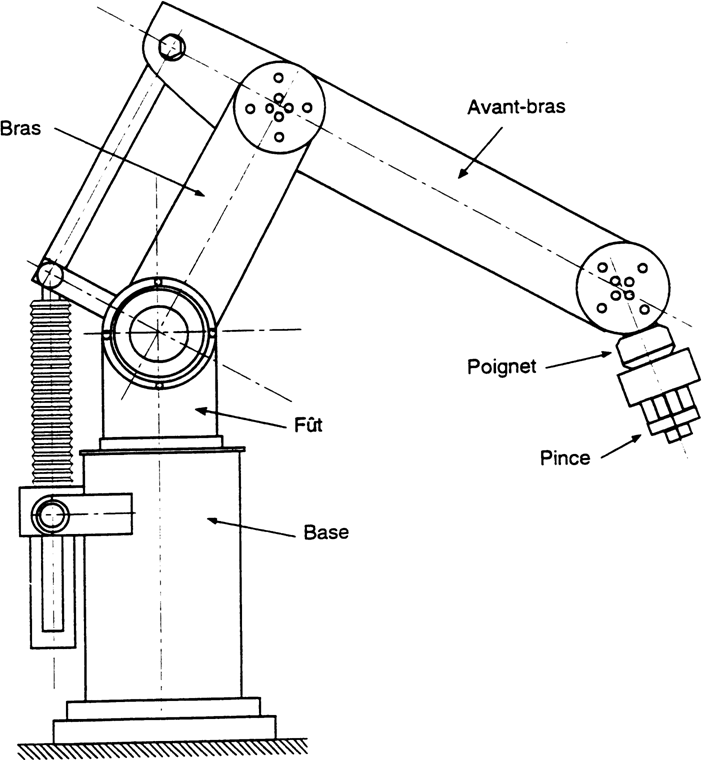
\includegraphics[width=\textwidth]{png/fig_01}
\end{center}
\end{minipage} \hfill
\begin{minipage}[c]{.65\linewidth}
Principales notations utilisées : 
\begin{itemize}
\item $J_m$ : inertie du moteur, du réducteur et de la charge;
\item $J_{me}$ : inertie globale équivalente sur l’arbre moteur;
\item $C_m$ : couple électromagnétique délivré par le moteur;
\item $C_{re}$ : couple résistant ramené sur l’arbre moteur ou couple équivalent;
\item $R$, $Ke$, $Kt$ : constantes électriques du moteur (résistance de l’induit, constante 	de force contre électromotrice et constante de couple);
\item $N$ : rapport de réduction;
\item $\omega_m$, $\theta_m$ : vitesse et position angulaire du moteur;
\item $\omega_c$, $\theta_c$ : vitesse et position angulaire de la charge.
\end{itemize}
\end{minipage}

On se propose tout d’abord d’étudier le modèle du moteur à vide c’est à dire du moteur seul : dans un premier temps par un modèle théorique et dans un second temps par une étude expérimentale. Ensuite il sera fait mention de la charge puis de la réalisation de l’asservissement de position.


\subsubsection*{Étude théorique du moteur seul}


Le moteur retenu pour animer la rotation du fût par rapport à la base est un servomoteur PARVEX de type AXEM à induit plat qui présente l’avantage de posséder une très faible inertie. C’est un moteur à courant continu.

Le comportement électromécanique de ce moteur dans l’hypothèse où l’inductance est négligeable, est donné par les équations suivantes :

\begin{eqnarray*}
u(t)=Ri(t)+e(t) \\
C_m(t)=K_t i(t) \\
e(t)= K_e \omega_m(t) \\
J_m \dfrac{d\omega_m (t)}{dt} = C_m(t)
\end{eqnarray*}





\subparagraph{}
\textit{En faisant l’hypothèse de conditions initiales sont nulles, calculez la transformée de Laplace $\Omega(m)$ en fonction de la transformée de Laplace $U(p)$.}

\ifthenelse{\boolean{prof}}{
\begin{corrige}
\end{corrige}
}{}


\subparagraph{}
\textit{Mettez le résultat sous la forme $\Omega_m(p)=\dfrac{K_m}{1+T_m p} U_m(p)$ en précisant $K_m$ et $T_m$.}

\ifthenelse{\boolean{prof}}{
\begin{corrige}
\end{corrige}
}{}


Les données du constructeur permettent de connaître les valeurs suivantes : $K_e=25,5\; V/(1000\; tr/min))$, $K_t=0,244 \; Nm/A$, $R=0,46\, \Omega$.



\subparagraph{}
\textit{Faites un calcul approché permettant de déterminer $K_m$ et $T_m$ ($T_m$  sera fonction de $J_m$  pour l’instant non connu).}

\ifthenelse{\boolean{prof}}{
\begin{corrige}
\end{corrige}
}{}

\textit{Remarque : pour toutes les applications numériques utilisez des unités S.I.}



\subsubsection*{Étude pratique du moteur seul}

Afin de valider le modèle précédent et de déterminer l’inertie du rotor du moteur on effectue une étude expérimentale sous la forme de l’observation de la réponse du moteur seul soumis à un échelon de tension de 50 V. Le résultat de cet essai est donné sur la courbe suivante.

\begin{center}
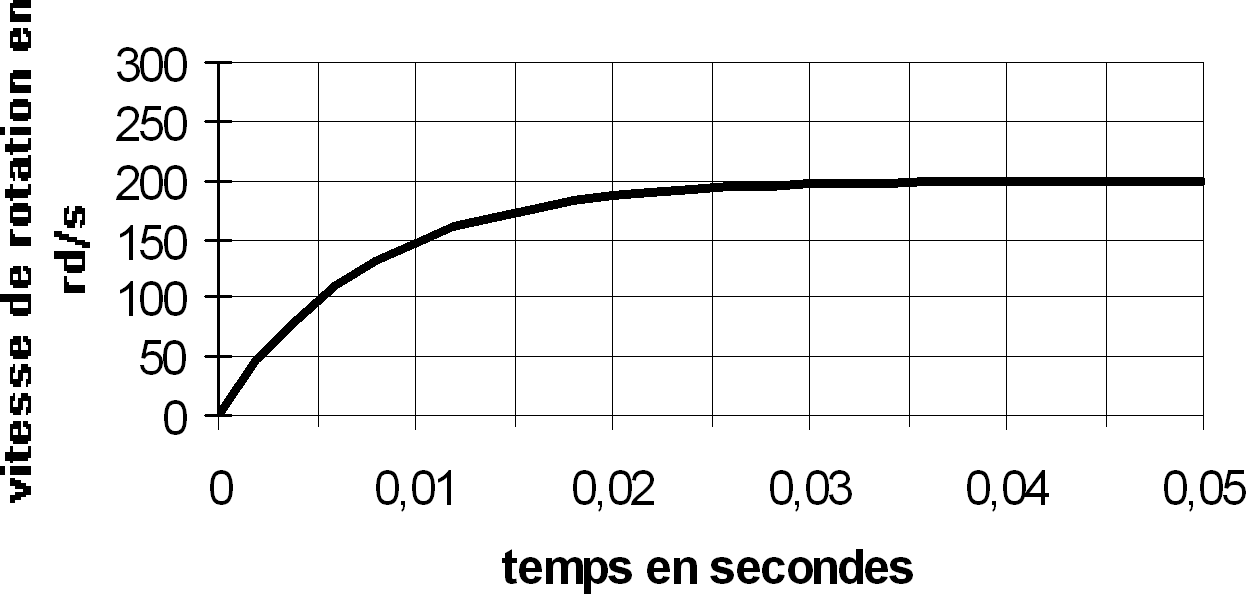
\includegraphics[width=.5\textwidth]{png/fig_02}
\end{center}

\subparagraph{}
\textit{Cette courbe est-elle bien conforme au modèle du premier ordre de la question précédente ? Pourquoi ?}

\ifthenelse{\boolean{prof}}{
\begin{corrige}
\end{corrige}
}{}

\subparagraph{}
\textit{Déterminez les valeurs expérimentales de $K_m$ et $T_m$. Déduisez-en la valeur expérimentale de $J_m$. }

\ifthenelse{\boolean{prof}}{
\begin{corrige}
\end{corrige}
}{}


\subsubsection*{Motorisation complète avec réducteur et charge}

La charge que devra entraîner le moteur est maintenant prise en compte ainsi que le réducteur qui permet de réduire la vitesse $\omega_m$ de rotation du moteur. En sortie du réducteur la vitesse de rotation est $\omega_c$.

L’inertie du moteur seule $J_m$ devient $J_{me}$ inertie équivalente de l’ensemble  charge + moteur + réducteur.

La charge crée un couple résistant équivalent $C_{re}$. On obtient donc l’équation suivante :
$$
C_m(t)=J_{me}\dfrac{d\omega_m(t)}{dt} + C_{re}(t)
$$



\subparagraph{}
\textit{A partir des équations électriques du moteur et de l’équation précédente, exprimez la transformée $\Omega_m(p)$. Les dénominateurs seront mis sous la forme $(1+T_{me} p)$. On précisera l’expression de $T_{me}$.}

\ifthenelse{\boolean{prof}}{
\begin{corrige}
\end{corrige}
}{}

\subparagraph{}
\textit{A partir du résultat précédent complétez le schéma fonctionnel suivant et explicitez clairement $G_1$, $G_2$, $G_3$, $G_4$. $G_3$ sera exprimé sous la forme d’un premier ordre avec pour constante de temps $T_{me}$.}

\begin{center}
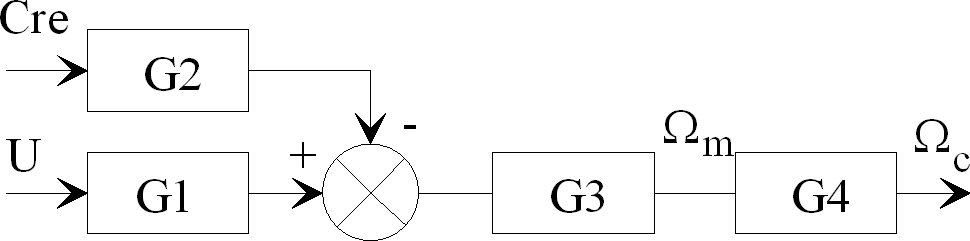
\includegraphics[width=0.5\textwidth]{png/fig_03}
\end{center}


\subsubsection*{Asservissement de position}

Pour la suite on suppose $C_{re}(p)$  nul. 

 Pour assurer l’asservissement de position angulaire du fût du robot (la sortie est alors un angle exprimé en radian), on associe au moteur un variateur de gain pur $K_a$ placé avant $G_1$ et on met en place un capteur de position angulaire de gain unitaire. Le capteur prendra l’information de position après le réducteur.



\subparagraph{}
\textit{Faites le schéma fonctionnel de l’asservissement ainsi constitué.}

\ifthenelse{\boolean{prof}}{
\begin{corrige}
\end{corrige}
}{}

\subparagraph{}
\textit{Calculez sa fonction de transfert. Donnez-en une interprétation pratique.}

\ifthenelse{\boolean{prof}}{
\begin{corrige}
\end{corrige}
}{}



\subsection*{Identification des systèmes d'ordre 1}

\subparagraph*{}
\textit{Pour chacune des courbes suivantes, donner l'expression de la fonction de transfert.}

\begin{minipage}[c]{.49\linewidth}
\begin{center}
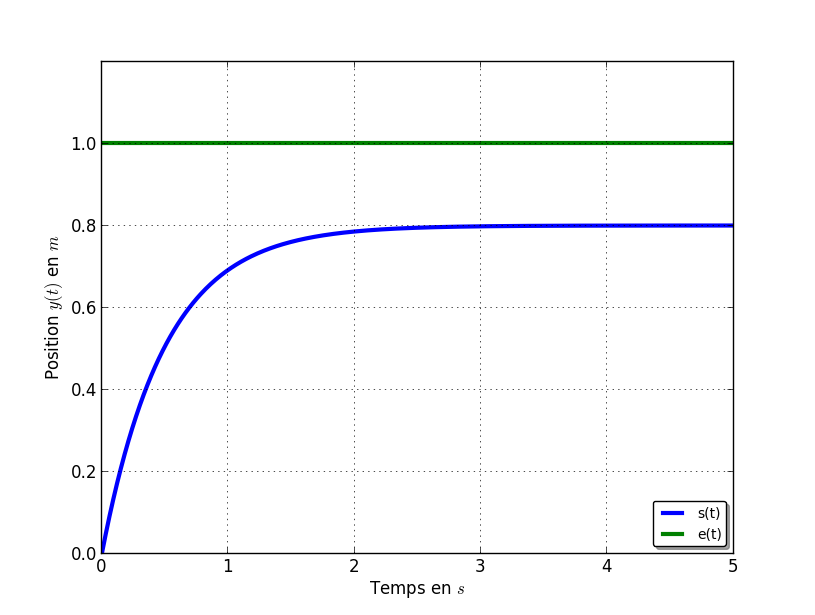
\includegraphics[width=\textwidth]{png/courbe1}
\end{center}
\end{minipage}\hfill
\begin{minipage}[c]{.49\linewidth}
\begin{center}
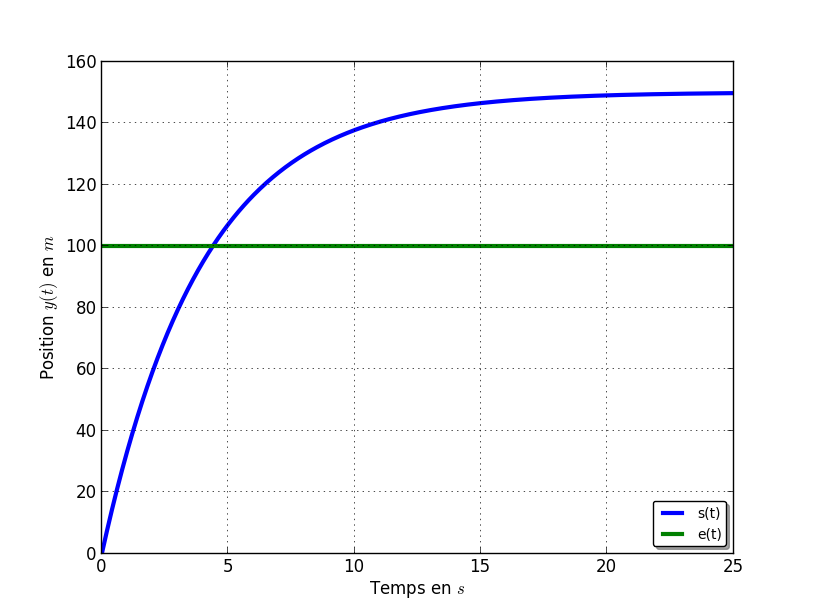
\includegraphics[width=\textwidth]{png/courbe2}
\end{center}
\end{minipage}

\begin{minipage}[c]{.49\linewidth}
\begin{center}
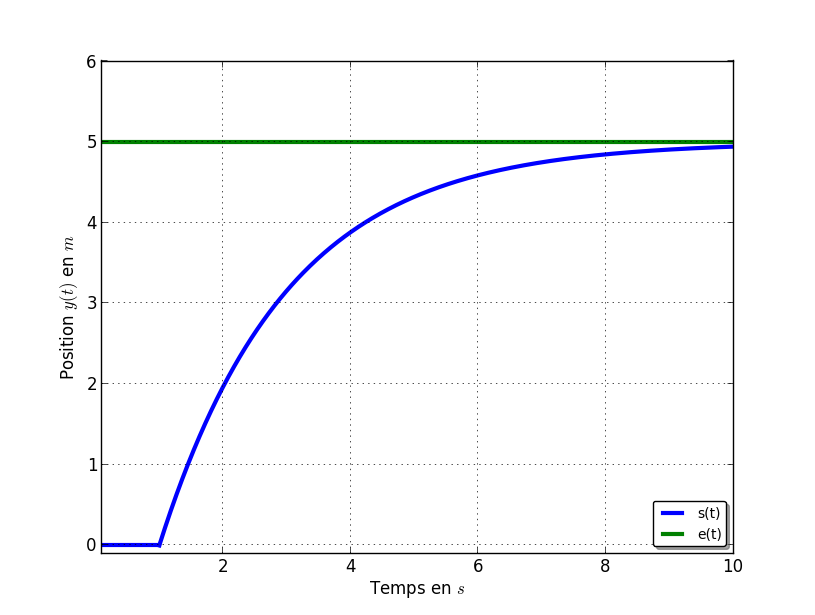
\includegraphics[width=\textwidth]{png/courbe3}
\end{center}
\end{minipage}\hfill
\begin{minipage}[c]{.49\linewidth}
\begin{center}
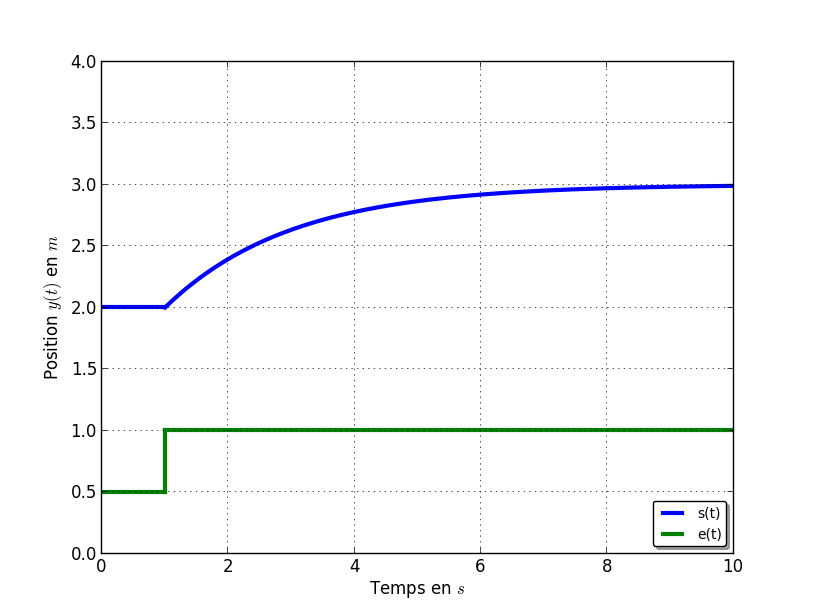
\includegraphics[width=\textwidth]{png/courbe4}
\end{center}
\end{minipage}




\end{document}
\subparagraph{}
\textit{}

\ifthenelse{\boolean{prof}}{
\begin{corrige}
\end{corrige}
}{}

\subparagraph{}
\textit{}

\ifthenelse{\boolean{prof}}{
\begin{corrige}
\end{corrige}
}{}

\subparagraph{}
\textit{}

\ifthenelse{\boolean{prof}}{
\begin{corrige}
\end{corrige}
}{}


